\section{Цепь №2 (<<Масштабный усилитель без инверсии фазы>>)}

\sidefig(0.5\textwidth){
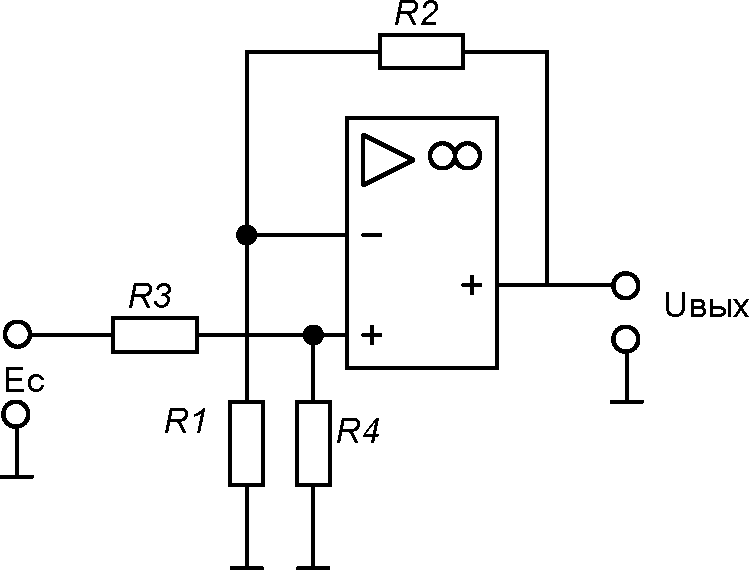
\includegraphics[scale=0.6]{Circ2.pdf}
\caption{Схема}
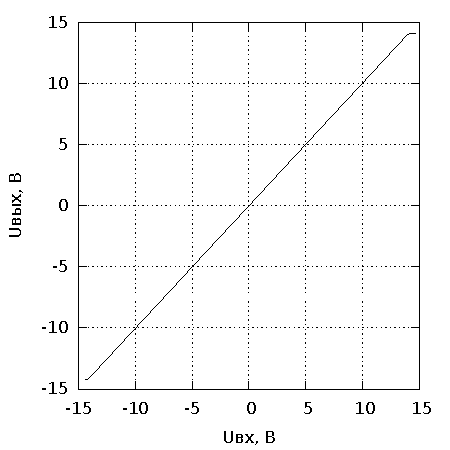
\includegraphics[scale=1.2]{4.pdf}
\caption{Для постоянного тока}}
{Табл. 4: Для постоянного тока

\small
\begin{tabular}{|l|l|l|}
\hline
$U_{вх}$, В & $U_{вых}$, В & K \\
\hline
-14.4&-14.2&0.99\\
\hline
-14.36&-14.21&0.99\\
\hline
-14.2&-14.2&1\\
\hline
-14.12&-14.13&1\\
\hline
-13.83&-13.86&1\\
\hline
-12.93&-12.95&1\\
\hline
-10.21&-10.23&1\\
\hline
-7.08&-7.1&1\\
\hline
-4.72&-4.72&1\\
\hline
-1.43&-1.43&1\\
\hline
-1.02&-1.02&1\\
\hline
-0.44&-0.44&1\\
\hline
-0.19&-0.2&1.05\\
\hline
0.19&0.19&1\\
\hline
0.57&0.57&1\\
\hline
0.97&0.97&1\\
\hline
1.3&1.3&1\\
\hline
2.49&2.5&1\\
\hline
5.08&5.09&1\\
\hline
7.49&7.51&1\\
\hline
9.82&9.83&1\\
\hline
12.77&12.79&1\\
\hline
13.94&13.96&1\\
\hline
14.01&14.03&1\\
\hline
14.23&14.1&0.99\\
\hline
14.38&14.1&0.98\\
\hline
14.72&14.11&0.96\\
\hline
\end{tabular}}

\sidefig(0.5\textwidth){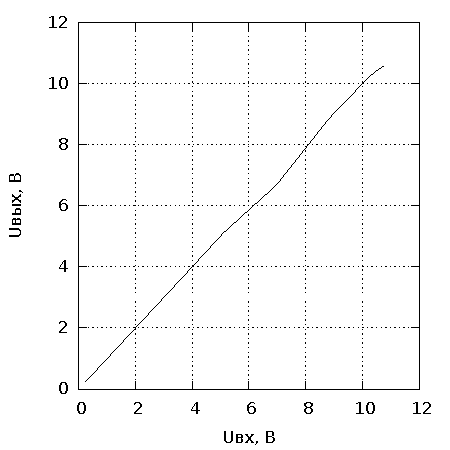
\includegraphics[scale=1.2]{5.pdf}
\caption{Для переменного тока}}
{Табл. 5: Для переменного тока

\begin{tabular}{|l|l|l|}
\hline
$U_{вх}$, В & $U_{вых}$, В & K \\
\hline
0.22&0.23&1.05\\
\hline
0.58&0.58&1.00\\
\hline
0.94&0.94&1.00\\
\hline
1.34&1.34&1.00\\
\hline
1.89&1.89&1.00\\
\hline
3.74&3.74&1.00\\
\hline
5.1&5.11&1.00\\
\hline
6.97&6.68&0.96\\
\hline
8.82&8.85&1.00\\
\hline
10.24&10.22&1.00\\
\hline
10.45&10.38&0.99\\
\hline
10.69&10.53&0.99\\
\hline
10.73&10.57&0.99\\
\hline
10.74&10.56&0.98\\
\hline
\end{tabular}}

\section{Цепь №3 (<<Усилитель переменного тока>>)}
\sidefig(0.4\textwidth){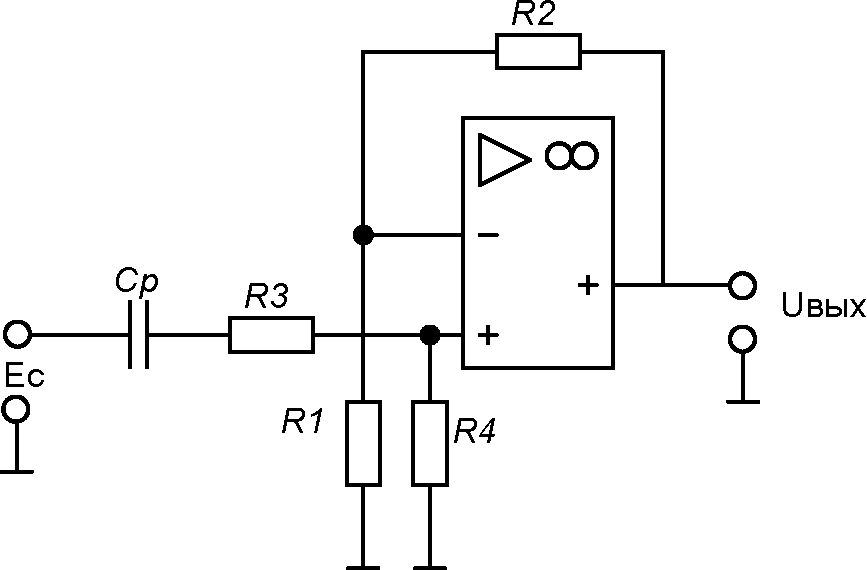
\includegraphics[scale=0.55]{Circ3.pdf}
\caption{Схема}}
{Табл. 6: ЛАЧХ усилителя

\begin{tabular}{|l|l|l|l|l|l|}
\hline
$f$, Гц & $U_{вх}$, В & $U_{вых}$, В & $K$ & $20\lg K$, дБ \\
\hline
16&4.6&0.12&0.03&-31.672\\
\hline
32&4.55&0.26&0.06&-24.861\\
\hline
64&4.51&0.52&0.12&-18.763\\
\hline
128&4.61&1.07&0.23&-12.686\\
\hline
256&4.58&1.97&0.43&-7.328\\
\hline
512&4.48&3.07&0.69&-3.283\\
\hline
1024&3.98&3.58&0.90&-0.920\\
\hline
2048&4.48&4.33&0.97&-0.296\\
\hline
4096&4.42&4.39&0.99&-0.059\\
\hline
8192&4.41&4.4&1.00&-0.020\\
\hline
16384&4.48&4.49&1.00&0.019\\
\hline
32768&4.21&4.22&1.00&0.021\\
\hline
65536&4.19&4.29&1.02&0.205\\
\hline
131072&3.97&4.05&1.02&0.173\\
\hline
209000&3.93&2.7&0.69&-3.261\\
\hline
\end{tabular}}

\begin{figure}[H]
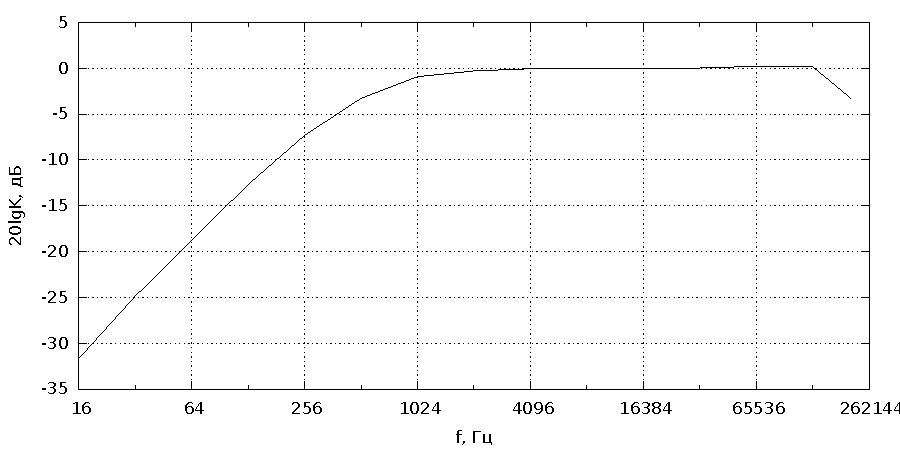
\includegraphics[scale=1]{6.pdf}
\caption{ЛАЧХ усилителя}
\end{figure}